% System / contract diagram: one outer loop, one Tesseract interface,
% three swappable framework-agnostic components.
% Compile:   pdflatex system_architecture.tex
% Rasterize: pdftoppm -png -r 300 system_architecture.pdf raw \
%            && magick raw-1.png -trim +repage system_architecture.png
\documentclass{article}
\usepackage[paperwidth=22cm, paperheight=12cm, margin=3mm]{geometry}
\usepackage{tikz}
\usepackage{amsmath}
\usepackage{amssymb}
\usepackage{bm}
\usetikzlibrary{positioning, arrows.meta, backgrounds, fit, calc}
\pagestyle{empty}

% Shared brand palette (refined light)
\definecolor{cLoop}{HTML}{2B3A47}    % ink slate (outer loop)
\definecolor{cBar}{HTML}{44566C}     % slate (contract bar)
\definecolor{cSolver}{HTML}{0E6E6E}  % deep teal (solver)
\definecolor{cPinn}{HTML}{3D3D9E}    % indigo (PINN)
\definecolor{cFmpe}{HTML}{9E2B3A}    % crimson (posterior)
\definecolor{cGrad}{HTML}{B5760A}    % amber (gradient / VJP)

\begin{document}
\noindent
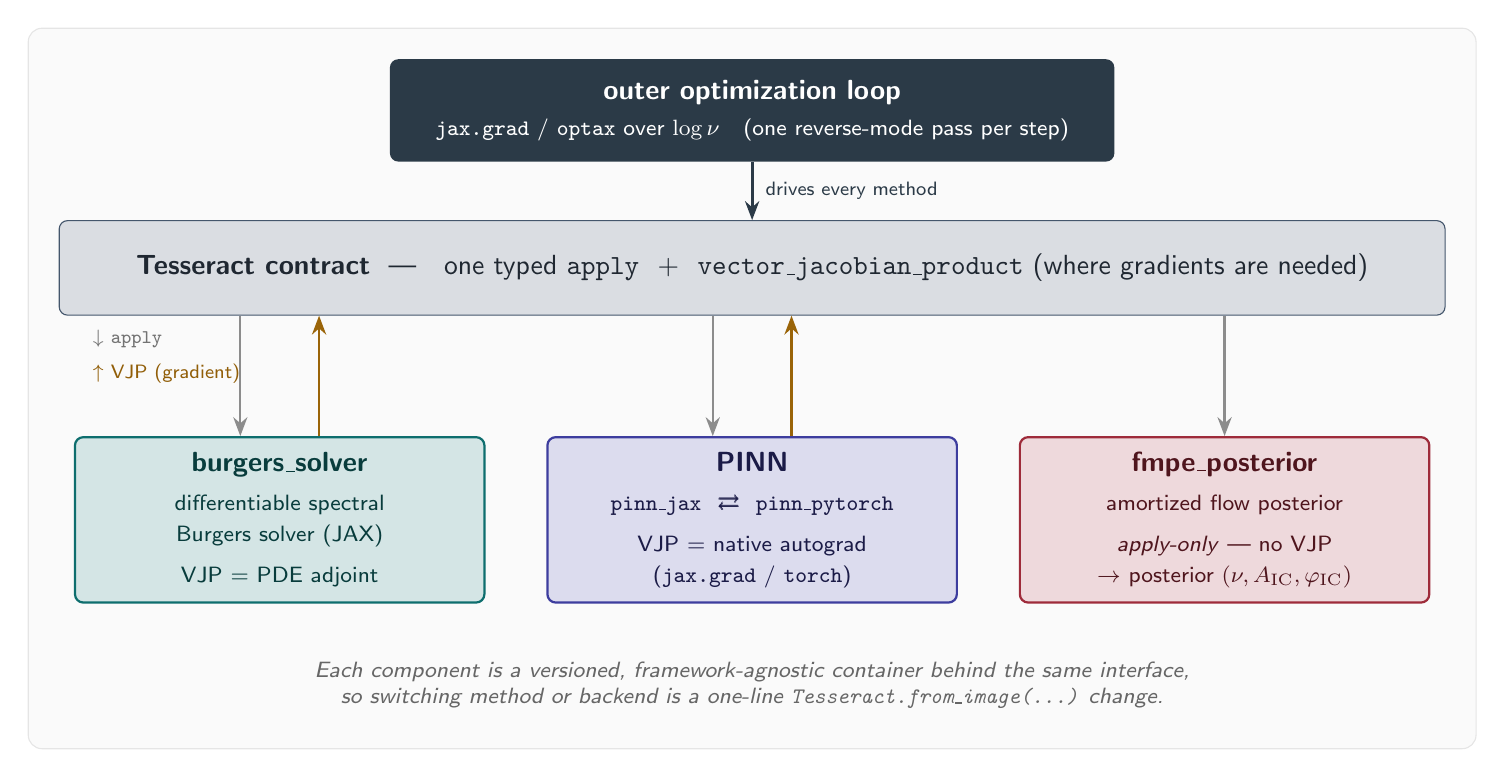
\begin{tikzpicture}[
  font=\sffamily,
  >={Stealth[length=2.4mm]},
  comp/.style={rounded corners=3pt, draw=black!45, line width=0.8pt,
               align=center, minimum width=52mm, minimum height=21mm,
               inner sep=5pt},
  applyarr/.style={->, draw=black!45, line width=0.8pt},
  vjparr/.style={->, draw=cGrad!85!black, line width=0.9pt},
  tag/.style={font=\sffamily\scriptsize, text=black!55},
]

% ---- Outer loop --------------------------------------------------------
\node[rounded corners=3pt, fill=cLoop, text=white, align=center,
      minimum width=92mm, minimum height=13mm, inner sep=5pt] (loop) at (9,5.4)
  {\textbf{outer optimization loop}\\[1pt]
   \footnotesize\texttt{jax.grad} / \texttt{optax} over $\log\nu$ \ \ (one
   reverse-mode pass per step)};

% ---- Tesseract contract bar -------------------------------------------
\node[rounded corners=3pt, fill=cBar!20, draw=cBar, text=cBar!45!black,
      align=center, minimum width=176mm, minimum height=12mm, inner sep=4pt]
      (bar) at (9,3.4)
  {\textbf{Tesseract contract}\ \ --- \ \ one typed
   \texttt{apply}\ \ $+$\ \ \texttt{vector\_jacobian\_product} (where gradients
   are needed)};

\draw[applyarr, draw=cLoop, line width=1pt] (loop) -- (bar)
  node[midway, right=1pt, tag, text=cLoop] {drives every method};

% ---- Three swappable components ---------------------------------------
\node[comp, fill=cSolver!18, draw=cSolver, text=cSolver!55!black] (solver) at (3,0.2)
  {\textbf{burgers\_solver}\\[2pt]
   \footnotesize differentiable spectral\\[-1pt]
   \footnotesize Burgers solver (JAX)\\[3pt]
   \footnotesize VJP $=$ PDE adjoint};

\node[comp, fill=cPinn!18, draw=cPinn, text=cPinn!45!black] (pinn) at (9,0.2)
  {\textbf{PINN}\\[2pt]
   \footnotesize\texttt{pinn\_jax}\ \ $\bm{\rightleftarrows}$\ \ \texttt{pinn\_pytorch}\\[3pt]
   \footnotesize VJP $=$ native autograd\\[-1pt]
   \footnotesize (\texttt{jax.grad} / \texttt{torch})};

\node[comp, fill=cFmpe!18, draw=cFmpe, text=cFmpe!50!black] (fmpe) at (15,0.2)
  {\textbf{fmpe\_posterior}\\[2pt]
   \footnotesize amortized flow posterior\\[3pt]
   \footnotesize \emph{apply-only} --- no VJP\\[-1pt]
   \footnotesize $\rightarrow$ posterior $(\nu, A_{\mathrm{IC}}, \varphi_{\mathrm{IC}})$};

% ---- apply (down) / VJP (up) connectors -------------------------------
\foreach \c in {solver, pinn} {
  \draw[applyarr] ($(\c.north |- bar.south) + (-0.5,0)$)
        -- ($(\c.north) + (-0.5,0)$);
  \draw[vjparr]   ($(\c.north) + (0.5,0)$)
        -- ($(\c.north |- bar.south) + (0.5,0)$);
}
% fmpe: apply only (centered)
\draw[applyarr] (fmpe.north |- bar.south) -- (fmpe.north);

% small legend for the two arrow directions, in the gap below the contract bar
\node[tag, anchor=west] at (0.5,2.5) {$\downarrow$ \texttt{apply}};
\node[tag, anchor=west, text=cGrad!80!black] at (0.5,2.06) {$\uparrow$ VJP (gradient)};

% ---- swappability caption ---------------------------------------------
\node[font=\sffamily\footnotesize\itshape, text=black!60, align=center]
  (cap) at (9,-1.9)
  {Each component is a versioned, framework-agnostic container behind the same
   interface,\\ so switching method or backend is a one-line
   \texttt{Tesseract.from\_image(...)} change.};

\begin{scope}[on background layer]
  \node[rounded corners=5pt, fill=black!2, draw=black!10,
        fit=(loop)(bar)(solver)(fmpe)(cap), inner sep=11pt] {};
\end{scope}

\end{tikzpicture}
\end{document}
